\section{PU의 스펙트럼 사용유무를 감지하는 머신러닝 모델의 labeling 방법}
    인지 무선 통신\footnote{Cognitive Radio} 기술은 사용하지 않고 있는 주파수 스펙트럼을 SDR \footnote{Software defined radio} 기반의 인공지능으로 감지하여 지역별,시간대별로 미사용 주파수를 인지하여 상황에 맞게 효율적으로 채널을 변경하여 사용하는 기술이다.
    
    스펙트럼 센싱은 PU\footnote{Primary User, 1차 사용자, 주파수 사용자}의 이용 현황을 감지하는 것으로 인지 무선 통신에서  기본 조건이 주파수 공유이지만 이미 해당주파수 자원을 할당 받아서 사용하는 이용자(PU)에게는 간섭을 주어서는 안되는 제약조건이 있기 떄문에 PU가 해당 spectrum 대역을 탐색하는 스펙트럼 센싱 방법이 필요하다. 
    
    이번 실험에 진행될 CNN 기반의 분류기를 이용한 스펙트럼 센싱적용을 위한 방법론을 조사해보고자 한다.  
\subsection{Cognitive Radio (인지 무선 통신)}
    \subsubsection*{Problem}
    \textbf{주사용자 (primary user, PU)}가 통신을 하지 않을 때 \textbf{부사용자 (secondary user, SU)}가 주사용자의 주파수 자원을 활용하여 통신하는 방법으로 정확하게 PU의 존재여부를 파악하는 스펙트럼 센싱의 방법론에 대한 문제.\\
        \begin{figure}[!h]\centering
    		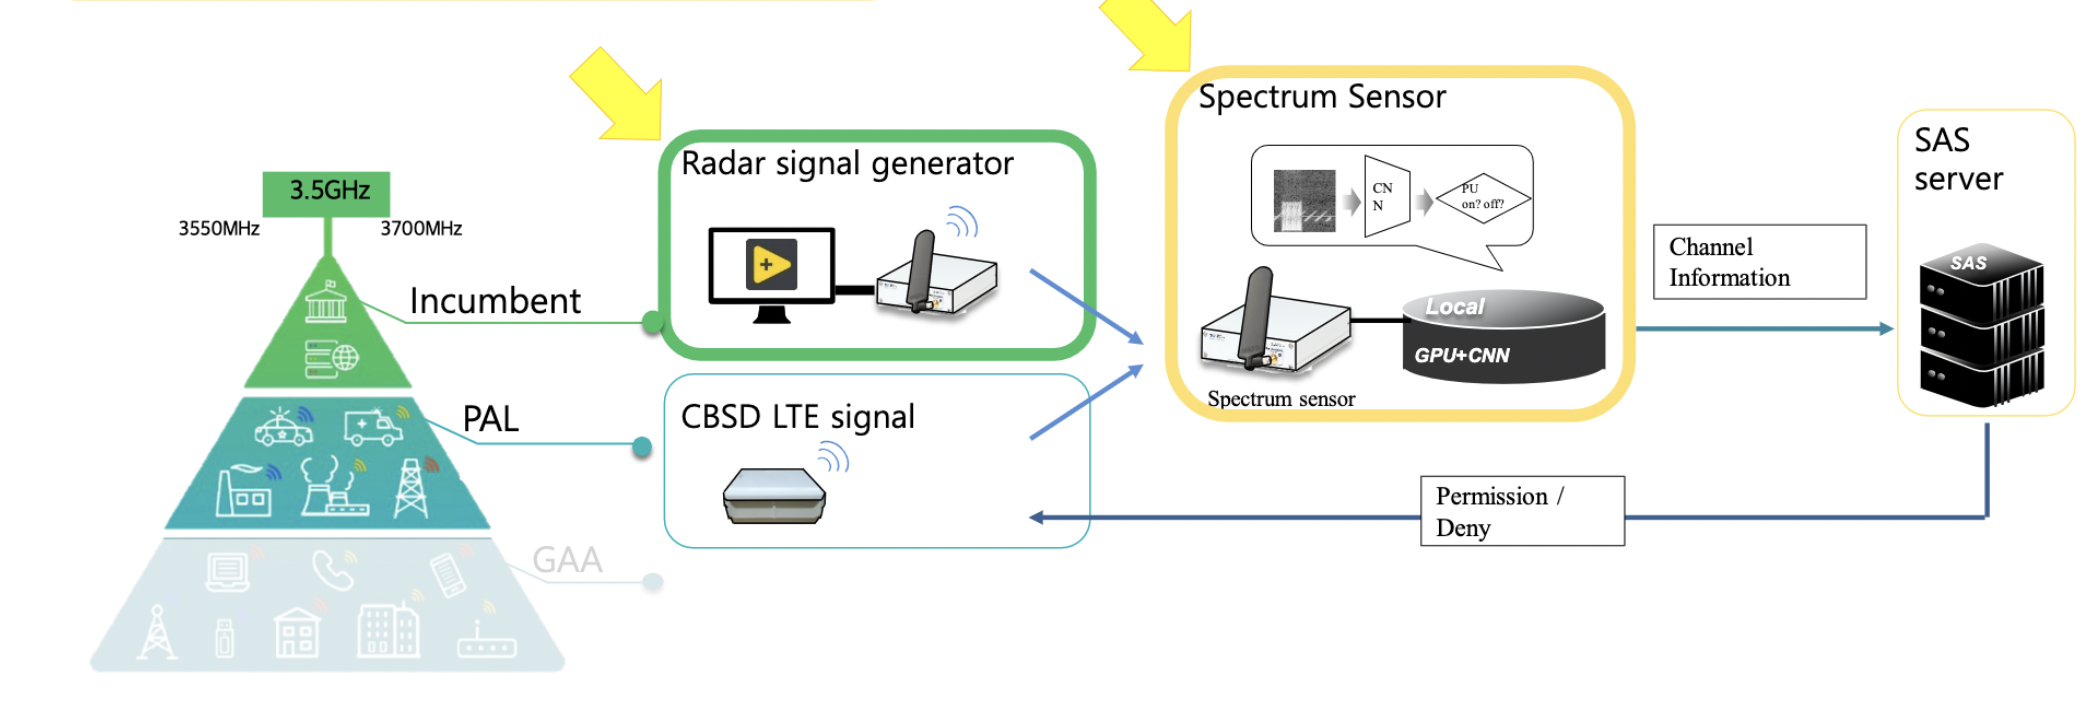
\includegraphics[width=.85\textwidth]{image/week04/4-0.png}
    		\caption{\small A roadmap for building machine learning systems}
    		\vspace{-10pt}
        \end{figure}
    \subsubsection*{Method}
    PU 신호의 정보에 대한 사전정보의 유무에 따른 방법론이 나뉜다. 
    \begin{itemize}
        \item PU 신호의 사전정보를 아는 경우 
        \item PU 산호의 사정정보를 모르는 경우
        \begin{itemize}
            \item 여러 SU들이 협력해서 PU의 존재를 펀단하는 스펙트럼 센싱기술 
            \item 에너지 검출 기법
        \end{itemize}
    \end{itemize}
    \subsubsection*{Spectrum Sensing : 에너지 검출 기법}
    \begin{itemize}
        \item 잡음의 전력을 추정하고 이를 기반으로 문턱 값을 설정한 후 수신신호의 전력이 문턱 값을넘으면 PU 신호가존재하고 그렇지않으면 PU 신호가 없는 것으로 판단
        \item 잡음의 전력값이 정확한 경우 준수한 성능을 보이지만, 정확하지 않은 경우 정확도가 떨어진다. 즉 잡음전력의 추정에 따라 분류기의 성능이 결정
    \end{itemize}
\clearpage
\subsection{에너지 검출 기법에 기반한 CNN 판별기의 스펙트럼 센싱}
    문제는 특정 주파수 스펙트럼대역 내부에서 PU 신호의 존재 유무로 labeling 하는것이다. 기존의 에너지 검출 방법과 같이 추정한 문턱신호의 출력값을 통하여 PU 신호가 존재하고 그렇지 않으면 PU 신호가 없는것으로 판단하는 접근법을 이용할 수 있다.
    
    수신신호의 크기 제곱을 CNN에 입력하고 CNN이 PU 신호의 존재의 유무를 판단하는 방법으로 labeling이 가능할 것이다. 세부 방법은 다음과 같다.
    \begin{enumerate}
        \item 센싱하고자 하는 전체 대역을 고려하여 수신신호를 고속으로 샘플링
        \item 스펙트럼 센싱을 위해 수신신호의 FFT(fast Fourier transform)를 통해 주파수 스펙트럼으로 변환하고 연속 적으로 수신한 신호에 대해서 스펙트럼을 구하고 쌓아서 2차원신호를 만든다.
        \item 만들어진 2차원 신호를 탐지하고자 하는 채널의 대역폭으로 자르고 각 채널 대역폭에 할당되지 않은 채널의 신호를 덧붙여 최종신호를 만들고 이를 CNN에 입력한다. 
        \item CNN은 분류하고자 하는 신호가 2종류 뿐이므로 이진분류신경망을 이용해 PU 신호의 존재를 판단한다. 
    \end{enumerate}
    % \vspace{-4mm}
    \begin{figure}[!h]\centering
		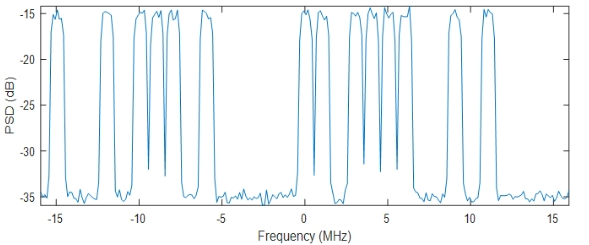
\includegraphics[width=.6\textwidth]{image/week04/4-1.png}
		\caption{\small주파수 스펙트럼에서 여러 channel의 PU 신호들이 관측되는것을 확인할 수 있다. }
		\vspace{-10pt}
    \end{figure}
    
    에너지 검출에 기반한 분류모델의 labeling의 과정을 수신신호모델을 예시로 어떻게 수행되는지 정리해 보았다.
\subsection{에너지 검출 기법에 기반한 CNN 판별기의 스펙트럼 센싱}
\subsubsection*{수신모델}
    \begin{figure}[!h]\centering
		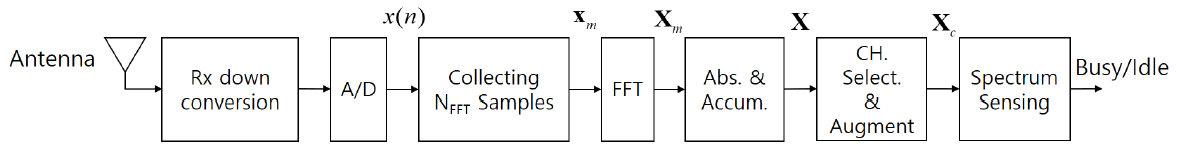
\includegraphics[width=.7\textwidth]{image/week04/4-2.png}
		\caption{\small스펙트럼 센싱 시스템 모델 }
		\vspace{-10pt}
    \end{figure}
    \begin{enumerate}
        \item 안테나를 통해서 수집된 신호가 ADC에 의해서 digital signal로 변환이 된다. 이 신호를 $x(n)$ 이라고 하자.
        \item$x(n)$ 은 FTT 크기인 $N_{FTT}$ 단위로 읽는데, 인접한 $N_{FTT}$개의 신호를 읽을때 오버랩하여 수집한다.\\
            \vspace{-4mm}
            \begin{figure}[!h]\centering
    		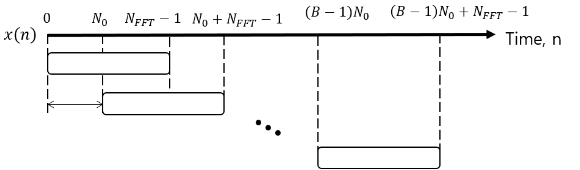
\includegraphics[width=.65\textwidth]{image/week04/4-3.png}
    		\caption{\small$x(n)$ 을 오버랩 하면서 신호를 취하는 과정 \newline
                $N_0$ 는 다음 신호를 취할 때 첫 sample 의 편이기간을 의미하며, 전체 신호 블록의 개수는 $B$ 이다.  }
    		\vspace{-10pt}
            \end{figure}
        \clearpage
        \item 여기서 $m+1$ 번째 수집신호 블록은 아래와 같이 표현할 수 있다.
            $$
            \mathbb{X}_m = \left [{x}(mN_0), \cdots, x(mN_0 + N_{FTT} -1)
            \right] \quad \text{for } m=0,\cdots,B-1
            $$
        \item PU 신호의 존재의 유무를 판단하기 위해서는 Time domain 보다는 Frequency domain 에서 스펙트럼을 통해 판단하는것이 유리하기 때문에, 앞서 수집한 sample을 FFT를 통해서 스펙트럼으로 변환한다.\\
        $x_m$ 의 $N_{FTT}$ 포인트 FTT 를 $\hat{X}_m$ 이라고 정의하자.
            $$
            \hat{X}_m = FTT\{x_m\} = [X_m(0), \cdots,X_m(N_{FTT} -1)]^T
            $$
        \item 에너지 검출기법에 기반한 스펙트럼 센싱기법을 사용하기 때문에  스펙트럼의 크기를 이용하여 판단을 해야 하므로 $\hat{X}_m$ 의 $N_{FTT}$ 개 원소에 대한 절대 값을 취해 준다. 
            $$
            |\hat{X}_m| \left [
            |\hat{X}_m(0)|, \cdots, |\hat{X}_m(N_{FTT} -1)|
            \right ]^{T
            }
            $$
        \item 총 $B$ 개의 신호블록에 대해서 각각 FTT를 수행하고 절대값을 취하여 $N_{FTT}$ by $B$ 의 Matrix 를 만들어서 $X$ 의 랜덤변수를 선언해 줄 수 있다. 
            $$
            X = \left [
            |\hat{X}_0|,\ |\hat{X}_1|, \cdots ,\ |\hat{X}_{B-1}| 
            \right ]
            $$
    \end{enumerate}
\subsubsection*{전처리된 신호에 대한 CNN 적용방법}
\begin{enumerate}
    \item $X$ 의 크기는 $N_{FTT} \timse B$ 의 2차원 행렬이며 CNN에 입력하기 위해서 각 channel 별로 분류가 필요하다. 
        \begin{itemize}
            \item 센싱채널폭을 $K_c$ 포인트라고 하자.
            \item 총 센싱채널의 개수는 $N_{FTT} / K_c$ 가 된다. 
            \item ADC 의 sampling clock 을 $F_s$ 라고 할때 각 센싱채널의 bandwidth는 $K_c\ F_s / N_{FTT}$ (Hz) 가 된다.
        \end{itemize}
    \item 센싱 channel의 전력과 잡음전력을 비교하여 PU signal의 존재를 판단한다.  $X$ 를 센싱채널별로 분류하고, 각 채널별로 채널에 잡음채널을 추가해 $X_c$를 만들어 준다. 
        $$
        X_c = 
        \left [
        \begin{matrix}
        \tilde{X}_c \\
        \tilde{X}_{N_{FTT} / K_c -1}
        \end{matrix}
        \right] \quad
        \text{for } c = 0, \cdots, N_{FTT}/K_c -2
        $$
        \begin{itemize}
            \item $X_c$ 를 CNN에 입력하여 PU 존재의 유무를 판단한다. 
            \item $\tilde{X}_c$는 크기 $K_c \times B$ 인 $X$의 부분행렬으로 $c K_c$ 부터 $(c+1) K_c - 1 $ 까지의 행을 선택한 것, $\tilde{X}_{N_{FTT} / K_c -1}$ 는 마지막 센싱채널로 항상 잡음이 있는 가정을 가져 잡음을 표현 
            \item 따라서 CNN에 Input 으로 들어가는 $X_c$ 의 size 는 $2 K_c \times B$  이다. 
        \end{itemize}
    \item (cf) 기존의 에너지 검출방식에서는 생성한 $X_c$ matrix에서 다음의 방법으로  수신신호의 전력을 측정하고 측정한 threshold를 기준으로 PU의 존재 여부를 판단한다. 
        $$
        \text{PU signal 유 무의 판단} \quad
        \begin{cases}
        \text{BUSY} & \hat{P}_c > \lambda\ (\text{threshold})\\
        \text{IDLE} & o.w.
        \end{cases}
        $$
        \begin{itemize}
            \item 수신신호 ($c + 1$) 번째 channel의 전력추정 값
                $$
                \hat{P}_c = \cfrac{1}{K_c B}\sum_{n=0}^{B-1}\sum_{m=0}^{K_c -1}
                \left |\tilde{X}_c (m,n)
                \right |^2
                $$
            \item PU의 유무를 판단하는 문턱값 $\lambda$ 는 noise channel의 추정값으로부터 구할 수 있다.
                \begin{align*}
                    \lambda &= \alpha \times \hat{P}_{\text{noise}} 
                    \quad (\footnotesize \alpha \text{ 는 SNR의 결정변수})\\
                    &= \alpha \times 
                    \cfrac{1}{K_c B}\sum_{n=0}^{B-1}\sum_{m=0}^{K_c -1}
                    \left |\tilde{X}_{N_{FTT}/K_c-1} (m,n)
                    \right |^2
                \end{align*}
        \end{itemize}
    \item 다시 에너지 검출에 기반한 CNN 접근법으로 돌아오자 \\ 
    결정해야 될것은 PU의 존재로 $\footnotesize \text{BUSY}$ 또는 $\footnotesize \text{IDLE}$ 로 labeling을 해주는, 최종적으로 fully connected layer 가 이진 분류신경망으로 구성해주면 된다. 
\clearpage
    \begin{figure}[!h]\centering
	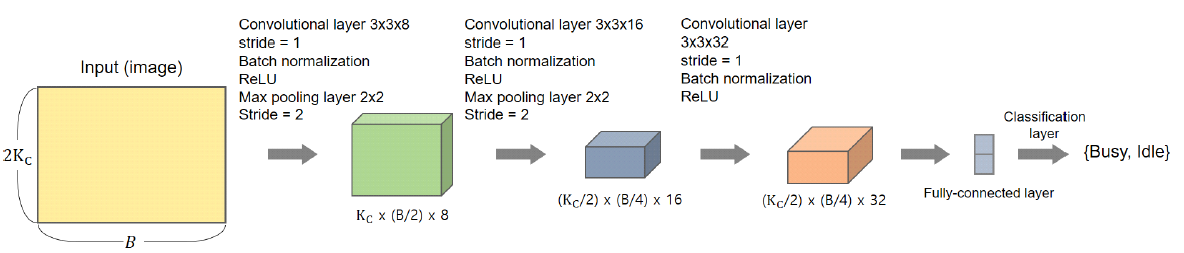
\includegraphics[width=.9\textwidth]{image/week04/4-4.png}
	\caption{\small Example CNN network for spectrum sensing}
	\vspace{-10pt}
    \end{figure}
    
    
\end{enumerate}